\chapter{Quantifying MGXS Approximations}
\label{chap:biases}

As discussed in Chapter~\ref{chap:mgxs}, a number of approximations are made in the multi-group formulation of the neutron transport equation and the \ac{MGXS} generation process. These approximations remain even if one uses the ``true'' scalar flux for energy condensation and spatial homogenization, as is the case with energy condensation and spatial homogenization in Monte Carlo\footnote{By the Law of Large Numbers, the \ac{MC} flux will be exactly correct in the limit of an infinite number of particle histories, though it is only a ``noisy'' proxy for a finite number of particles.}. The observed bias between a continuous energy \ac{MC} and a multi-group deterministic calculation reflects the convolution of these approximations, which may (or may not) lead to some degree of fortuitous cancellation of error. Although this thesis is motivated by the need for \ac{MGXS} for whole-core calculations, it is instructive to investigate the approximations inherent in multi-group theory and quantify their impact for simple benchmark models.

In this chapter, a series of case studies is devised to systematically quantify biases inherent to the energy condensation and spatial homogenization process(es) in multi-group transport theory. The results underline the complex interactions between discretizations in energy, space and angle. Various convergence studies with respect to each of these variables are presented to quantify the resulting magnitude of the bias induced between continuous energy Monte Carlo and multi-group deterministic calculations. The results in this chapter illustrate the loss in accuracy resulting from scalar flux-weighted total \ac{MGXS} due to the flux separability approximation (see Sec.~\ref{subsec:chap2-angle}), and highlight the need for models of the angular dependency in \ac{MGXS} for fine mesh deterministic neutron transport. Finally, this chapter verifies the data pipeline used to compute multi-group cross sections with OpenMC for use in OpenMOC (see Chap.~\ref{chap:workflow}).


%%%%%%%%%%%%%%%%%%%%%%%%%%%%%%%%%%%%%%%%%%%%%%%%%%%%%%%%%%%%%%%%%%%%%%%%%%%%%%%%
\section{Case Studies}
\label{sec:chap5-case-studies}

This chapter investigates the loss in accuracy resulting from approximations made in both the \ac{MOC} equations as well as the \ac{MGXS} generation scheme with OpenMC. The benchmarks are designed to illustrate the emergence of the approximation errors as spatial heterogeneity is introduced in the geometric models. The approximation errors are quantified for a variety of geometric and material configurations based on a standard \ac{PWR}. In each case, the bias $\Delta\rho$ compares the eigenvalue $k_{eff}^{OpenMOC}$ computed with \ac{MGXS} in OpenMOC to that of the reference eigenvalue $k_{eff}^{OpenMC}$ computed with continuous energy cross sections in OpenMC in units of \ac{pcm}:

\begin{equation}
\label{eqn:chap5-delta-rho}
\Delta\rho = \left(k_{eff}^{OpenMOC} - k_{eff}^{OpenMC}\right) \times 10_{5}
\end{equation}

In each case study, the role of angular discretization in \ac{MOC} is quantified through convergence studies of the number of azimuthal angles and the track spacing used in the deterministic \ac{MOC} calculations. The effects of energy discretization are analyzed for \ac{MGXS} tallied in the CASMO~\cite{rhodes2006casmo} energy group structures ranging from 1 -- 70 groups (see App.~\ref{app:energy-groups}). For each of the case studies with heterogeneous geometries, the spatial domain is discretized in OpenMOC's \ac{FSR} mesh with constant-by-material \ac{MGXS} to quantify the interaction between the energy and spatial approximations. Spatial discretization studies show the impact of tallying \ac{MGXS} in each of the \ac{FSR}s used in the discretized OpenMOC geometry. Finally, \ac{MGXS} libraries were tallied using OpenMC's iso-in-lab feature (see Sec.~\ref{subsec:chap4-iso-in-lab}) to quantify the impact of the isotropic in lab scattering approximation used in OpenMOC. Inter-pin spatial self-shielding effects are not treated here as they are studied in detail in Chaps.~\Crefrange{chap:benchmarks}{chap:unsupervised}. In each case study, OpenMOC was converged to a criterion of 10$_{-7}$ on the energy-integrated fission source in each \ac{FSR}.

%%%%%%%%%%%%%%%%%%%%%%%%%%%%
\subsection{Homogeneous Infinite Medium}
\label{subsec:chap5-inf-medium}

An initial series of case studies were performed for a homogeneous infinite medium problem. The isotopic composition of the infinite medium was a homogenized mixture derived from the 1.6\% enriched UO$_2$ \ac{PWR} fuel pin in the \ac{BEAVRS} \ac{PWR} model~\cite{horelik2013beavrs} and is described in Tab.~\ref{table:chap5-inf-med-isotopes}. No approximation is made in the multi-group formulation of the transport equation in the case of homogeneous infinite media. As a result, neutron balance should be exactly preserved within numerical precision in deterministic calculations with \ac{MGXS} computed in any energy group structure, assuming the \ac{MC} tallies used to compute \ac{MGXS} are sufficiently converged.

\begin{table}[h!]
  \centering
  \caption[Infinite medium isotopic composition]{Homogeneous infinite medium isotopic composition.}
  \small
  \label{table:chap5-inf-med-isotopes} 
  \vspace{6pt}
  \begin{tabular}{c c}
  \toprule
  \rowcolor{lightgray}
  {\bf Nuclide} &
  {\bf Density [atom / b-cm]} \\
  \midrule
  H-1 &   4.12377E-2 \\
  O-16 &  2.06218E-2 \\
  Zr-90 & 3.00904E-3 \\
  U-235 & 1.62310E-4 \\
  U-238 & 9.79198E-3 \\
  \bottomrule
\end{tabular}
\end{table}

The reference eigenvalues computed with continuous energy cross sections in OpenMC are shown in Tab.~\ref{table:chap5-inf-med-reference} for both normal anisotropic as well as iso-in-lab scattering. As one would expect for a homogeneous infinite medium, the eigenvalues for anisotropic and iso-in-lab scattering agree to within one standard deviation of the mean. The reference calculations were computed for 100 batches of 10$_{8}$ particles per batch. The \texttt{openmc.mgxs} module was used to compute 70-group libraries of $\hat{\Sigma}_{t,g}$, $\hat{\Sigma}_{s,k,g'\rightarrow g}$, $\nu\hat{\Sigma}_{f,g}$, and $\hat{\chi}_{g}$ from OpenMC tallies (see Tab.~\ref{table:chap3-tally-types}).

\begin{table}[h!]
  \centering
  \caption[Reference $k^{OpenMC}_{\infty}$ for an infinite medium]{Reference $k^{OpenMC}_{\infty}$ for a homogeneous infinite medium.}
  \small
  \label{table:chap5-inf-med-reference} 
  \vspace{6pt}
  \begin{tabular}{c c}
  \toprule
  \rowcolor{lightgray}
  {\cellcolor{carolinablue} {\bf Anisotropic}} &
  {\cellcolor{lightgreen} {\bf Isotropic in Lab}} \\
  \midrule
  1.15908 $\pm$ 0.00001 & 1.15907 $\pm$ 0.00001 \\
  \bottomrule
\end{tabular}
\end{table}

%%%%%%%%%%%%%%%%%%%%%%%%%%%%%%%%%%%%%%%%%%%%%%%
\subsubsection{Angular Discretization}
\label{subsubsec:chap5-inf-med-angle}

The first case study investigated the sensitivity of the OpenMOC eigenvalue to the angular discretization used in the \ac{MOC} calculation. Tab.~\ref{table:chap5-inf-med-angle} presents the bias $\Delta\rho$ between OpenMC and OpenMOC for a matrix of azimuthal angles and track spacings. The results for both normal and iso-in-lab scattering indicate consistent agreement of the eigenvalues irregardless of track discretization. This result is expected since the neutron source is isotropic in homogeneous infinite media and does not depend on the angular discretization used to solve the eigenvalue problem.

\vspace{0.1in}

\begin{table}[h!]
  \centering
  \caption[Angular discretization error for an infinite medium]{Convergence study of the eigenvalue bias $\Delta\rho$ with varying azimuthal angle quadratures and track spacings for a homogeneous infinite medium.}
  \small
  \label{table:chap5-inf-med-angle}
  \vspace{6pt}
  \begin{tabular}{| q | S[table-format=4.1] S[table-format=4.1] S[table-format=4.1] | S[table-format=4.1] S[table-format=4.1] S[table-format=4.1] |}
  \hhline{~|------|}
  \multicolumn{1}{c|}{} &
  \multicolumn{6}{c|}{\cellcolor{lightgray} \bf Track Spacing [cm]} \\
  \multicolumn{1}{c|}{} &
  {\cellcolor{lightgray} \bf 0.1} &
  {\cellcolor{lightgray} \bf 0.01} & 
  \multicolumn{1}{S[table-format=4.1]}{\cellcolor{lightgray} {\bf 0.001}} &
  \multicolumn{1}{S[table-format=4.1]}{\cellcolor{lightgray} {\bf 0.1}} & 
  {\cellcolor{lightgray} \bf 0.01} & 
  \multicolumn{1}{S[table-format=4.1]|}{\cellcolor{lightgray} {\bf 0.001}} \\
  \midrule
  {\bf \# Angles} & \multicolumn{3}{c|}{\cellcolor{carolinablue} \bf Anisotropic} &
  \multicolumn{3}{c|}{\cellcolor{lightgreen} \bf Isotropic in Lab} \\
  \cline{2-7}
4 & 1.3 & 1.3 & 1.3 & -0.1 & -0.1 & -0.1 \\
8 & 1.3 & 1.3 & 1.3 & -0.1 & -0.1 & -0.1 \\
16 & 1.3 & 1.3 & 1.3 & -0.1 & -0.1 & -0.1 \\
32 & 1.3 & 1.3 & 1.3 & -0.1 & -0.1 & -0.1 \\
64 & 1.3 & 1.3 & 1.3 & -0.1 & -0.1 & -0.1 \\
128 & 1.3 & 1.3 & 1.3 & -0.1 & -0.1 & -0.1 \\
  \bottomrule
\end{tabular}
\end{table}

%%%%%%%%%%%%%%%%%%%%%%%%%%%%%%%%%%%
\subsubsection{Energy Condensation}
\label{subsubsec:chap5-inf-med-energy}

A second case study investigated the variation of the OpenMOC eigenvalue with the energy group structure used in the \ac{MOC} calculation. Tab.~\ref{table:chap5-inf-med-energy} presents the bias $\Delta\rho$ between OpenMC and OpenMOC for a matrix of energy group structures and \ac{FSR} spatial discretizations. The OpenMOC calculations each used 128 azimuthal angles and 0.01 cm track spacing. Although the eigenvalues differ by approximately 10 \ac{pcm} for 1 and 2 groups, the OpenMOC eigenvalues match the eigenvalues computed analytically from the 1- and 2-group \ac{MGXS} to within 1 pcm. The 10 \ac{pcm} bias may be due to numerical roundoff error since the \ac{MGXS} library was tallied in 70 groups in OpenMC and condensed to the coarser group structures with data processing  by the \texttt{openmc.mgxs} module.

\begin{table}[h!]
  \centering
  \caption[Energy discretization error for an infinite medium]{Convergence study of the eigenvalue bias $\Delta\rho$ with varying energy group structures for a homogeneous infinite medium.}
  \small
  \label{table:chap5-inf-med-energy} 
  \vspace{6pt}
  \begin{tabular}{| q | S[table-format=2.1] | S[table-format=2.1] |}
  \toprule
  {\bf \# Groups} &
  {\cellcolor{carolinablue} {\bf \hspace{0.3cm}Anisotropic\hspace{0.3cm}}} &
  {\cellcolor{lightgreen} {\bf Isotropic in Lab}} \\
  \cline{2-3}
1 & -11.1 & -10.5 \\
2 & -9.5 & -7.1 \\
4 & -0.1 & -0.5 \\
8 & 0.3 & -0.0 \\
16 & -0.2 & 0.5 \\
25 & 1.8 & 0.1 \\
40 & 1.6 & 0.1 \\
70 & 1.3 & -0.1 \\
  \bottomrule
\end{tabular}
\end{table}

\vspace{0.5cm}
\begin{emphbox}
\textbf{The eigenvalues for a homogeneous infinite medium agree to within nearly 10 \ac{pcm} for all \ac{MOC} angular discretizations and energy group structures.}
\end{emphbox}


%%%%%%%%%%%%%%%%%%%%
\subsection{1D Slab}
\label{subsec:chap5-slab}

A simple slab model was constructed to quantify approximation errors in a 1D heterogeneous geometry with spatial self-shielding. The slab model was constructed as an ``equivalent'' 1D model to the 2.4\% enriched UO$_2$ \ac{PWR} fuel pin in the \ac{BEAVRS} \ac{PWR} model~\cite{horelik2013beavrs}. The geometric configuration of UO$_2$ fuel, helium gap, zirconium clad and water moderator is illustrated in Fig.~\ref{fig:chap5-slab} and the dimensions for each material zone are shown in Tab.~\ref{table:chap5-slab-widths}. The width of each spatial region was chosen to preserve the volumetric fraction of each material in the slab with those in the corresponding 2D fuel pin\footnote{A truly ``equivalent'' slab would preserve the mean chord lengths of each material in the 2D fuel pin.}. Reflective boundary conditions were applied to all $x$, $y$ and $z$ boundaries in the geometry. The isotopic composition of each material in the slab is identical to the \ac{BEAVRS} fuel pin and is itemized in Tab.~\ref{table:chap5-slab-isotopes}. 

\begin{figure}[h!]
\begin{subfigure}{\textwidth}
  \centering
  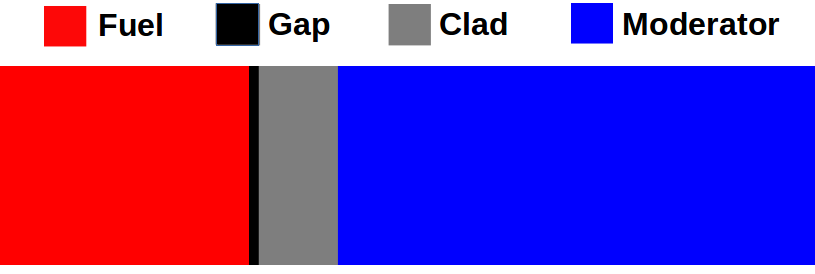
\includegraphics[width=0.7\linewidth]{figures/biases/slab/slab-simple-labels}
  \caption{}
  \label{fig:chap5-slab-a}
\end{subfigure} \\
\begin{subfigure}{\textwidth}
  \centering
  
\includegraphics[width=0.7\linewidth]{figures/biases/slab/slab-8x}
  \caption{}
  \label{fig:chap5-slab-b}
\end{subfigure}
\caption[1D slab materials and geometry]{A 1D slab with fuel, clad and moderator (a). Linearly-spaced tally zones were defined in the fuel and moderator in OpenMC and as \ac{FSR}s in OpenMOC (b).}
\label{fig:chap5-slab}
\end{figure}

\begin{table}[h!]
  \centering
  \caption[1D slab dimensions]{1D slab dimensions.}
  \small
  \label{table:chap5-slab-widths} 
  \vspace{6pt}
  \begin{tabular}{l c}
  \toprule
  \rowcolor{lightgray}
  \multicolumn{1}{c}{\bf Material} &
  \multicolumn{1}{c}{\bf Width [cm]} \\
  \midrule
  Fuel &  0.19177 \\
  Gap &   0.00777 \\
  Clad &  0.06109 \\
  Water & 0.36929 \\
  \bottomrule
\end{tabular}
\end{table}

\begin{table}[h!]
  \centering
  \caption[1D slab isotopic composition]{1D slab isotopic composition.}
  \small
  \label{table:chap5-slab-isotopes} 
  \vspace{6pt}
  \begin{tabular}{c c c}
  \toprule
  \rowcolor{lightgray}
  {\bf Material} &
  {\bf Nuclide} &
  {\bf Density [atom / b-cm]} \\
  \midrule
  \multirow{3}{*}{\bf UO$_2$} & O-16 &  4.58508E-2 \\
  & U-235 & 5.58415E-4 \\
  & U-238 & 2.24186E-2 \\
  \midrule
  \multirow{1}{*}{\bf Helium} & He-4 & 2.40428E-4 \\
  \midrule
  \multirow{3}{*}{\bf Zircaloy} & O-16 &  6.14041E-4 \\
  & Fe-56 & 2.71837E-4 \\
  & Zr-90 & 4.35958E-2 \\
  \midrule
  \multirow{4}{*}{\bf Water} & H-1 &  4.95774E-2 \\
  & B-10 & 8.02369E-6 \\
  & B-11 & 3.22964E-5 \\
  & O-16 & 2.47320E-2 \\
  \bottomrule
\end{tabular}
\end{table}

The reference eigenvalues computed with continuous energy cross sections in OpenMC are shown in Tab.~\ref{table:chap5-slab-reference} for both normal anisotropic as well as iso-in-lab scattering. The reference calculations were computed for 100 batches of 10$_{7}$ particles per batch. The reference eigenvalues for the two cases vary by nearly 75 \ac{pcm} due to anisotropies resulting from thermal scattering in the moderator. The \texttt{openmc.mgxs} module was used to compute 70-group libraries of $\hat{\Sigma}_{t,k,g}$, $\hat{\tilde{\Sigma}}_{t,k,g}$, $\hat{\Sigma}_{s,k,g'\rightarrow g}$, $\hat{\tilde{\Sigma}}_{s,k,g'\rightarrow g}$, $\nu\hat{\Sigma}_{f,g}$, and $\hat{\chi}_{g}$ from OpenMC tallies (see Tab.~\ref{table:chap3-tally-types}).

\begin{table}[h!]
  \centering
  \caption[Reference $k^{OpenMC}_{eff}$ for a 1D slab]{Reference $k^{OpenMC}_{eff}$ for a 1D slab.}
  \small
  \label{table:chap5-slab-reference} 
  \vspace{6pt}
  \begin{tabular}{c c}
  \toprule
  \rowcolor{lightgray}
  {\cellcolor{carolinablue} {\bf Anisotropic}} &
  {\cellcolor{lightgreen} {\bf Isotropic in Lab}} \\
  \midrule
  1.16275 $\pm$ 0.00003 & 1.16202 $\pm$ 0.00003 \\
  \bottomrule
\end{tabular}
\end{table}

%%%%%%%%%%%%%%%%%%%%%%%%%%%%%%%%%%%%%%%%%%%%%%%
\subsubsection{Angular Discretization}
\label{subsubsec:chap5-slab-angle}

The first case study investigated the convergence of the OpenMOC eigenvalue with the angular discretization used in the \ac{MOC} calculation. Tab.~\ref{table:chap5-slab-angle} presents the bias $\Delta\rho$ between OpenMC and OpenMOC for a matrix of azimuthal angles and track spacings. Two different 70-group \ac{MGXS} libraries were computed from OpenMC tallies with anisotropic and iso-in-lab scattering. No transport correction was applied to the total cross section $\hat{\Sigma}_{t,k,g}$ or the scattering matrix $\hat{\Sigma}_{s,k,g'\rightarrow g}$. No spatial discretization was applied to the materials for the \ac{FSR} mesh in OpenMOC. The results for anisotropic and iso-in-lab scattering exhibit a bias resulting from the multi-group approximation which converges to 170 and 280 pcm, respectively. The magnitude of the bias appears to converge with 128 azimuthal angles and was largely insensitive to the track spacing. The \ac{MGXS} tallied with iso-in-lab scattering in OpenMC eliminates the isotropic scattering approximation in OpenMOC but increases the overall bias by over 100 \ac{pcm} with respect to the anisotropic case due to the cancellation of other approximation errors.

\begin{table}[h!]
  \centering
  \caption[Angular discretization error for a 1D slab]{Convergence study of the 70-group eigenvalue bias $\Delta\rho$ with varying azimuthal angle quadratures and track spacings for a 1D slab.}
  \small
  \label{table:chap5-slab-angle}
  \vspace{6pt}
  \begin{tabular}{| q | S[table-format=6.1] S[table-format=6.1] S[table-format=6.1] | S[table-format=6.1] S[table-format=6.1] S[table-format=6.1] |}
  \hhline{~|------|}
  \multicolumn{1}{c|}{} &
  \multicolumn{6}{c|}{\cellcolor{lightgray} \bf Track Spacing [cm]} \\
  \multicolumn{1}{c|}{} &
  {\cellcolor{lightgray} \bf 0.1} &
  {\cellcolor{lightgray} \bf 0.01} & 
  \multicolumn{1}{S[table-format=6.1]}{\cellcolor{lightgray} {\bf 0.001}} &
  \multicolumn{1}{S[table-format=6.1]}{\cellcolor{lightgray} {\bf 0.1}} & 
  {\cellcolor{lightgray} \bf 0.01} & 
  \multicolumn{1}{S[table-format=6.1]|}{\cellcolor{lightgray} {\bf 0.001}} \\
  \midrule
  {\bf \# Angles} & \multicolumn{3}{c|}{\cellcolor{carolinablue} \bf Anisotropic} &
  \multicolumn{3}{c|}{\cellcolor{lightgreen} \bf Isotropic in Lab} \\
  \cline{2-7}
4 & 731 & 731 & 731 & 840 & 840 & 840 \\
8 & 472 & 339 & 323 & 581 & 448 & 432 \\
16 & 282 & 166 & 149 & 390 & 275 & 257 \\
32 & 154 & 135 & 131 & 262 & 243 & 239 \\
64 & 158 & 146 & 156 & 266 & 254 & 265 \\
128 & 165 & 164 & 169 & 274 & 272 & 278 \\
256 & 161 & 171 & 172 & 270 & 280 & 280 \\
512 & 165 & 170 & 172 & 274 & 278 & 281 \\
  \bottomrule
\end{tabular}
\end{table}

\newpage

%%%%%%%%%%%%%%%%%%%%%%%%%%%%%%%%%%%
\subsubsection{Energy Condensation and FSR Discretization}
\label{subsubsec:chap5-slab-energy}

The second case study investigated the variation of the OpenMOC eigenvalue with the energy group structure used in the \ac{MOC} calculation. This case study simultaneously varied the \ac{FSR} discretization used in the OpenMOC simulation. Tab.~\ref{table:chap5-slab-energy} presents the bias $\Delta\rho$ between OpenMC and OpenMOC for a matrix of energy group structures and \ac{FSR} spatial discretizations. In each case, the \ac{MGXS} used in OpenMOC were tallied by material in OpenMC (\textit{i.e.}, the spatial tally mesh corresponded to Fig.~\ref{fig:chap5-slab-a}). The OpenMOC calculations each used 128 azimuthal angles and 0.01 cm track spacing. The slab was discretized into 1 -- 16 equal volume \ac{FSR}s in the fuel and moderator.

\begin{table}[h!]
  \centering
  \caption[Energy and spatial discretization error for a 1D slab]{Convergence study of the eigenvalue bias $\Delta\rho$ with varying energy group structures and \ac{FSR} spatial discretizations for a 1D slab with \textit{\ac{MGXS} tallied by material}.}
  \small
  \label{table:chap5-slab-energy} 
  \vspace{6pt}
  \begin{tabular}{| q | S[table-format=6.1] S[table-format=6.1] S[table-format=6.1] S[table-format=6.1] S[table-format=6.1] |}
  \hhline{~|-----|}
  \multicolumn{1}{c|}{\cellcolor{white}} & \multicolumn{5}{c|}{\cellcolor{lightgray} {\bf \ac{FSR} Discretization}} \\
  \multicolumn{1}{c|}{\cellcolor{white}} &
  {\cellcolor{lightgray} {\bf 1$\times$}} &
  {\cellcolor{lightgray} {\bf 2$\times$}} &
  {\cellcolor{lightgray} {\bf 4$\times$}} &
  {\cellcolor{lightgray} {\bf 8$\times$}} &
  {\cellcolor{lightgray} {\bf 16$\times$}} \\
  \midrule
  \multicolumn{1}{|c|}{\cellcolor{lightgray} {\bf \# Groups}} & \multicolumn{5}{c|}{\cellcolor{carolinablue} \bf Anisotropic w/o Transport Correction} \\
  \hhline{~|-----|}
1 & 70 & 71 & 72 & 72 & 71 \\
2 & 106 & -16 & -80 & -101 & -85 \\
4 & 112 & -2 & -63 & -90 & -87 \\
8 & 158 & -13 & -109 & -149 & -160 \\
16 & 182 & -9 & -117 & -162 & -173 \\
25 & 146 & -37 & -143 & -190 & -201 \\
40 & 155 & -40 & -155 & -205 & -217 \\
70 & 164 & -38 & -156 & -208 & {\cellcolor{darktangerine}} -221 \\
  \midrule
  \multicolumn{1}{c|}{\cellcolor{white}} & \multicolumn{5}{c|}{\cellcolor{lightgreen} \bf Anisotropic w/ Transport Correction} \\
  \midrule
1 & 87 & 88 & 88 & 88 & 87 \\
2 & 285 & 211 & 175 & 167 & 189 \\
4 & 188 & 113 & 75 & 51 & 63 \\
8 & 211 & 81 & 13 & -23 & -24 \\
16 & 232 & 82 & 1 & -39 & -40 \\
25 & 148 & -1 & -89 & -123 & -128 \\
40 & 148 & -14 & -111 & -149 & -156 \\
70 & 153 & -16 & -118 & -158 & {\cellcolor{darktangerine}} -166 \\
  \midrule
  \multicolumn{1}{c|}{\cellcolor{white}} & \multicolumn{5}{c|}{\cellcolor{lightsalmonpink} \bf Isotropic in Lab} \\
  \midrule
1 & 132 & 134 & 135 & 135 & 133 \\
2 & 289 & 167 & 102 & 81 & 97 \\
4 & 226 & 112 & 50 & 24 & 26 \\
8 & 296 & 126 & 30 & -10 & -21 \\
16 & 321 & 131 & 22 & -22 & -33 \\
25 & 258 & 75 & -31 & -78 & -88 \\
40 & 262 & 67 & -47 & -98 & -110 \\
70 & 272 & 71 & -48 & -100 & {\cellcolor{darktangerine}} -113 \\
  \bottomrule
\end{tabular}
\end{table}

The results illustrate a strong interaction between the energy and spatial meshes used to solve the multi-group transport equation. The eigenvalue bias varies by up to 150 \ac{pcm} between energy group structures and nearly 400 \ac{pcm} between \ac{FSR} discretizations. The application of the transport correction reduces the bias by 55 \ac{pcm} for the 70-group structure and 16$\times$ \ac{FSR} discretization. The use of the iso-in-lab scattering feature reduces the bias by an additional 50 \ac{pcm} with respect to anisotropic scattering. 

\clearpage

%%%%%%%%%%%%%%%%%%%%%%%%%%%%%%%%%%%
\subsubsection{Spatial Homogenization and FSR Discretization}
\label{subsubsec:chap5-slab-space}

Finally, a case study was performed to investigate the sensitivity of the OpenMOC eigenvalue to the spatial tally mesh used to compute \ac{MGXS}. This study was identical to that presented in Sec.~\ref{subsubsec:chap5-slab-energy}, but the \textbf{\ac{MGXS} were computed using a tally mesh in OpenMC identical to the \ac{FSR} mesh used by OpenMOC}. Tab.~\ref{table:chap5-slab-space} presents the bias $\Delta\rho$ for a matrix of energy group structures and \ac{MGXS} spatial tally zone meshes. In each case, the \ac{MGXS} were tallied on the \ac{FSR} mesh with 1 -- 16 equal volume subdivisions in the fuel and moderator (\textit{i.e.}, the spatial tally mesh corresponded to Fig.~\ref{fig:chap5-slab-b}). The OpenMOC calculations each used 128 azimuthal angles and 0.01 cm track spacing.

\begin{table}[h!]
  \centering
  \caption[Spatial homogenization error for a 1D slab]{Convergence study of the eigenvalue bias $\Delta\rho$ with varying energy group structures and \ac{FSR} spatial discretizations for a 1D slab with \textit{\ac{MGXS} tallied by \ac{FSR}}.}
  \small
  \label{table:chap5-slab-space} 
  \vspace{6pt}
  \begin{tabular}{| q | S[table-format=6.1] S[table-format=6.1] S[table-format=6.1] S[table-format=6.1] S[table-format=6.1] |}
  \hhline{~|-----|}
  \multicolumn{1}{c|}{\cellcolor{white}} & \multicolumn{5}{c|}{\cellcolor{lightgray} {\bf \ac{FSR} Discretization}} \\
  \multicolumn{1}{c|}{\cellcolor{white}} &
  {\cellcolor{lightgray} {\bf 1$\times$}} &
  {\cellcolor{lightgray} {\bf 2$\times$}} &
  {\cellcolor{lightgray} {\bf 4$\times$}} &
  {\cellcolor{lightgray} {\bf 8$\times$}} &
  {\cellcolor{lightgray} {\bf 16$\times$}} \\
  \midrule
  \multicolumn{1}{|c|}{\cellcolor{lightgray} {\bf \# Groups}} & \multicolumn{5}{c|}{\cellcolor{carolinablue} \bf Anisotropic w/o Transport Correction} \\
  \hhline{~|-----|}
1 & 68 & 107 & 111 & 78 & 113 \\
2 & 104 & 9 & -63 & -107 & -82 \\
4 & 110 & 10 & -36 & -80 & -71 \\
8 & 156 & -11 & -86 & -144 & -141 \\
16 & 180 & -10 & -97 & -158 & -153 \\
25 & 144 & -39 & -127 & -180 & -173 \\
40 & 153 & -42 & -138 & -196 & -190 \\
70 & 162 & -39 & -142 & -202 & {\cellcolor{darktangerine}} -198 \\
  \midrule
  \multicolumn{1}{c|}{\cellcolor{white}} & \multicolumn{5}{c|}{\cellcolor{lightgreen} \bf Anisotropic w/ Transport Correction} \\
  \midrule
1 & 85 & 90 & 103 & 92 & 98 \\
2 & 283 & 213 & 189 & 167 & 201 \\
4 & 186 & 120 & 96 & 62 & 86 \\
8 & 209 & 84 & 26 & -19 & -11 \\
16 & 230 & 84 & 11 & -40 & -31 \\
25 & 146 & -3 & -82 & -125 & -118 \\
40 & 147 & -16 & -107 & -152 & -147 \\
70 & 152 & -19 & -114 & -161 & {\cellcolor{darktangerine}} -156 \\
  \midrule
  \multicolumn{1}{c|}{\cellcolor{white}} & \multicolumn{5}{c|}{\cellcolor{lightsalmonpink} \bf Isotropic in Lab} \\
  \midrule
1 & 139 & 97 & 127 & 162 & 140 \\
2 & 296 & 145 & 100 & 90 & 88 \\
4 & 233 & 125 & 77 & 61 & 51 \\
8 & 304 & 136 & 45 & 7 & -9 \\
16 & 329 & 139 & 38 & -6 & -23 \\
25 & 266 & 83 & -11 & -54 & -70 \\
40 & 270 & 75 & -29 & -73 & -89 \\
70 & 280 & 76 & -33 & -81 & {\cellcolor{darktangerine}} -93 \\
  \bottomrule
\end{tabular}
\end{table}

The trends analyzed in Tab.~\ref{table:chap5-slab-energy} emerge in a nearly identical manner with spatially-dependent\footnote{In this context, spatially-dependent refers to \ac{MGXS} defined on the \ac{FSR} rather than the material mesh.} \ac{MGXS} in Tab.~\ref{table:chap5-slab-space}. In particular, the eigenvalue bias grows in magnitude with more energy groups, and is largely invariant to \ac{FSR} spatial discretization or the elimination of the isotropic scattering approximation with iso-in-lab scattering. Most importantly, the results in Tab.~\ref{table:chap5-slab-space} indicate that spatial self-shielding effects (\textit{e.g.}, variations in the flux energy spectrum across the fuel) captured with spatially-dependent scalar flux-weighted \ac{MGXS} for each \ac{FSR} do not have a substantial impact on the systematic errors in the eigenvalue for this 1D slab problem.

\vspace{0.5cm}
\begin{emphbox}
\textbf{A systematic bias of -100 to -200 \ac{pcm} exists between OpenMC and OpenMOC for a 1D slab. The bias varies with the \ac{FSR} discretization and grows with more energy groups. The bias is partially eliminated with iso-in-lab scattering, and is largely invariant to the spatial mesh used to generate \ac{MGXS}.}
\end{emphbox}

\clearpage


%%%%%%%%%%%%%%%%%%%%%%%%%%%%%
\subsection{2D Fuel Pin Cell}
\label{subsec:chap5-pin}

A \ac{PWR} fuel pin cell model was constructed to quantify approximation errors in a 2D heterogeneous geometry with spatial self-shielding. The pin cell is identical to the 2.4\% enriched UO$_2$ \ac{PWR} fuel pin in the \ac{BEAVRS} \ac{PWR} model~\cite{horelik2013beavrs}. The geometric configuration of UO$_2$ fuel, helium gap, zirconium clad and water moderator is illustrated in Fig.~\ref{fig:chap5-pin-cell} and the dimensions for each material zone are shown in Tab.~\ref{table:chap5-pin-dimensions}. Reflective boundary conditions were applied to all boundaries in the geometry. The isotopic compositions of each material in the fuel pin were identical to those used in the 1D slab (see Tab.~\ref{table:chap5-slab-isotopes}). 

\begin{table}[H]
  \centering
  \caption[2D fuel pin dimensions]{2D fuel pin dimensions.}
  \label{table:chap5-pin-dimensions} 
  \vspace{6pt}
  \begin{tabular}{l c}
  \toprule
  \rowcolor{lightgray}
  \multicolumn{1}{c}{\cellcolor{lightgray} {\bf Material}} &
  {\bf Dimension [cm]} \\
  \midrule
  Fuel Outer Radius &     0.39218 \\
  Gap Outer Radius &      0.40005 \\
  Clad Outer Radius &     0.45720 \\
  Pin Pitch &             1.25984 \\
  \bottomrule
\end{tabular}
\end{table}

\begin{figure}[H]
\centering
\begin{subfigure}{.32\textwidth}
  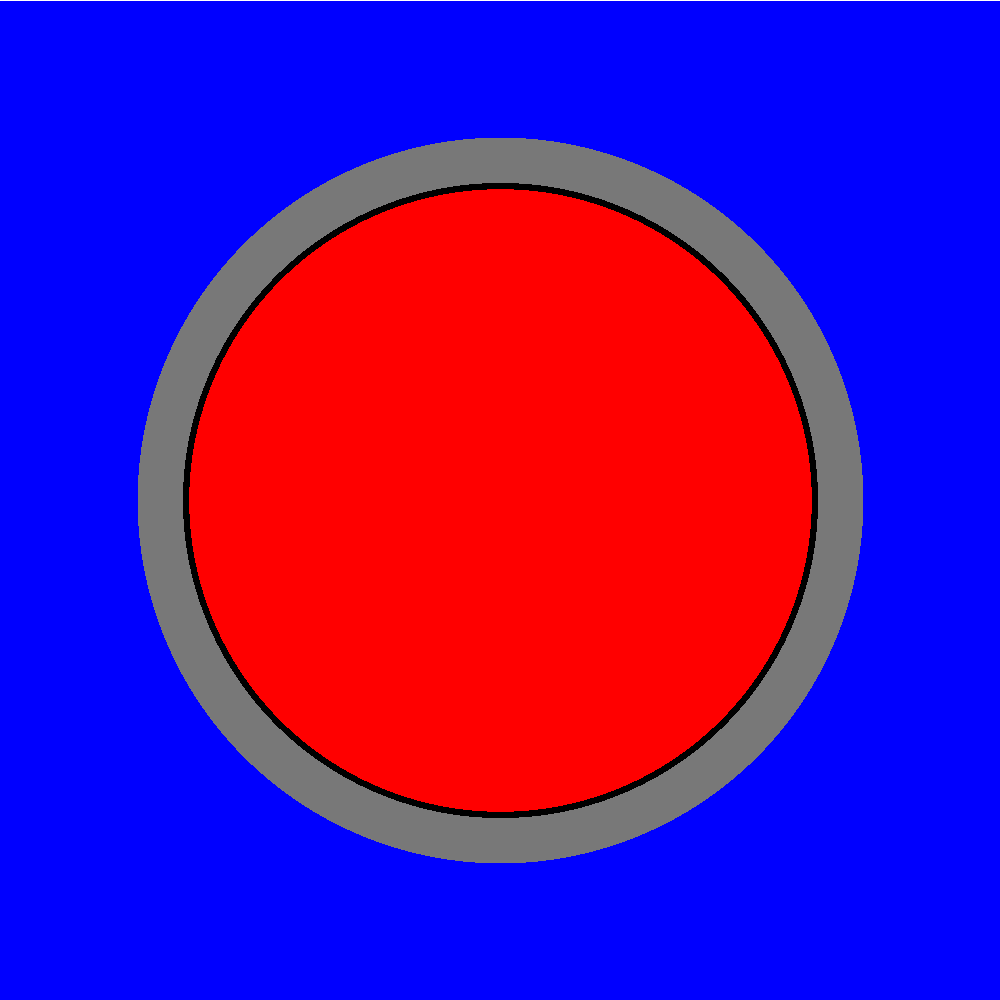
\includegraphics[width=0.9\linewidth]{figures/biases/pin-cell/pin-cell-simple}
  \caption{}
  \label{fig:chap5-pin-a}
\end{subfigure}%
\begin{subfigure}{.32\textwidth}
  \centering
  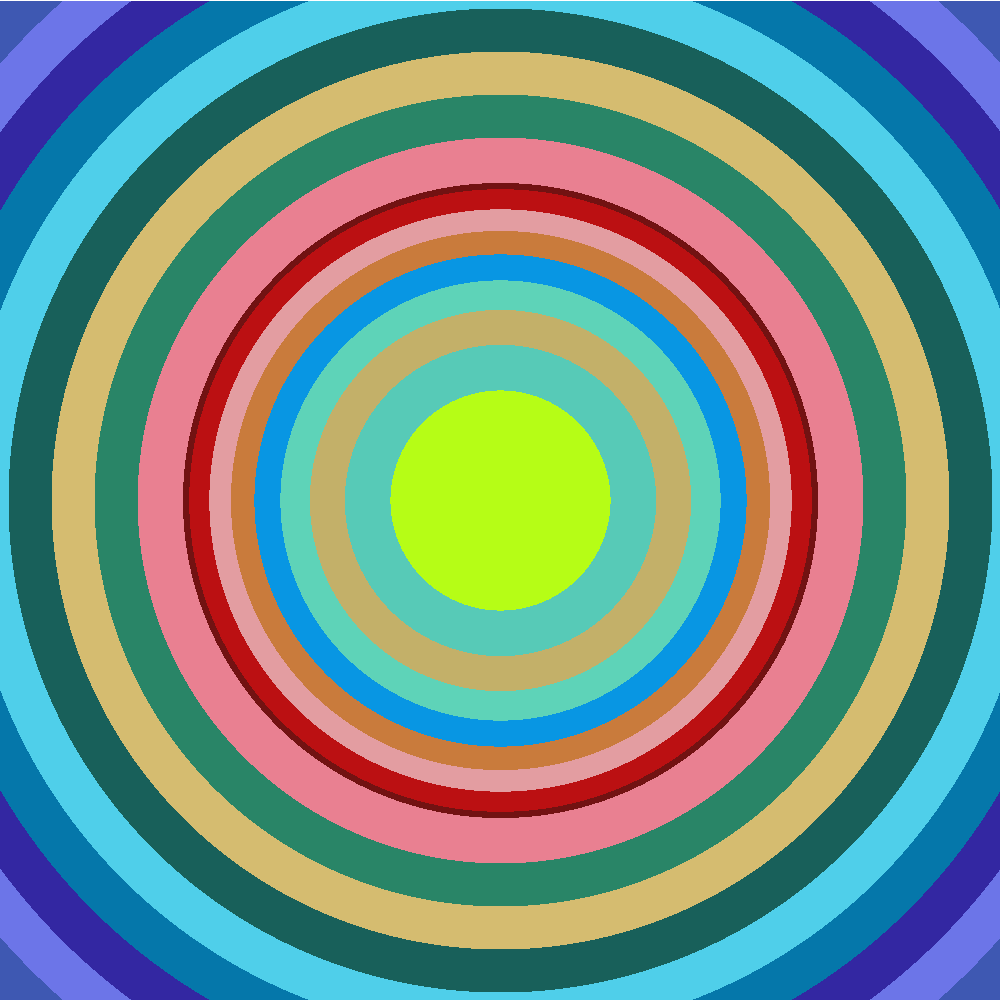
\includegraphics[width=0.9\linewidth]{figures/biases/pin-cell/pin-cell-8x}
  \caption{}
  \label{fig:chap5-pin-b}
\end{subfigure}
\begin{subfigure}{.32\textwidth}
  \centering
  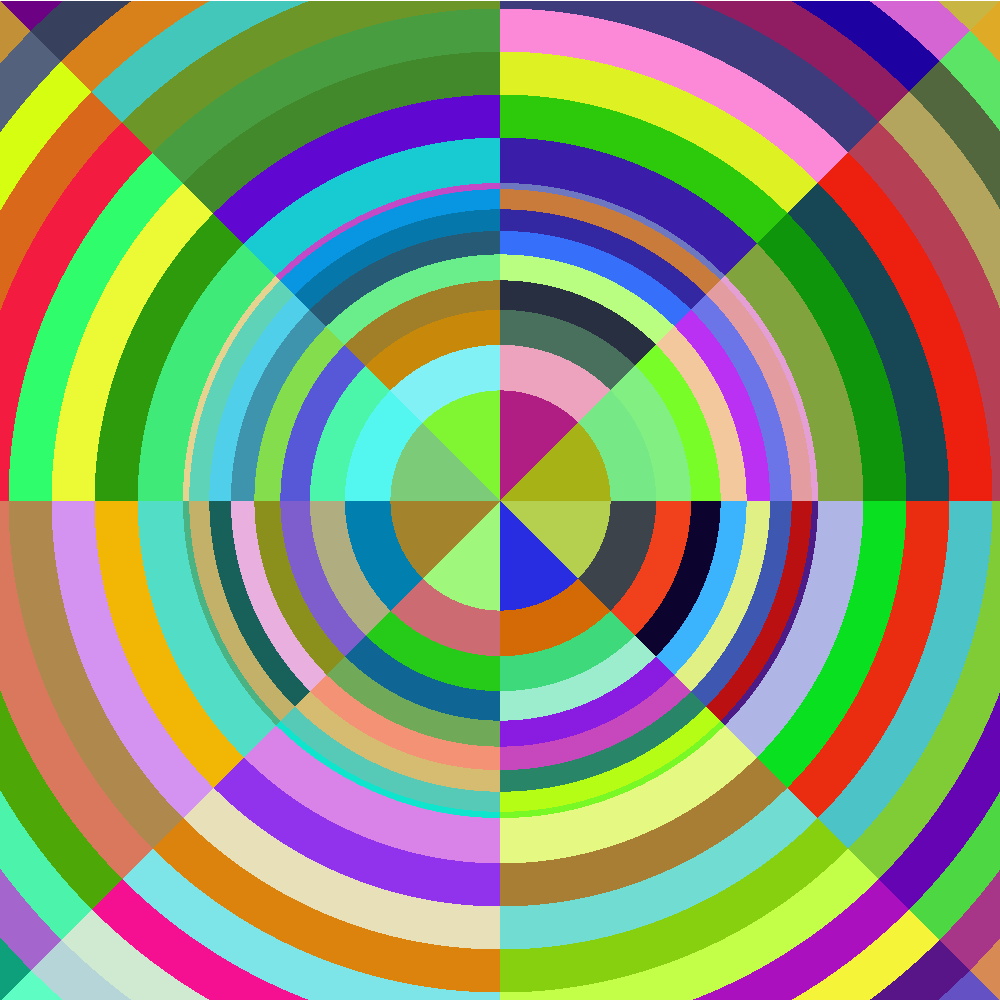
\includegraphics[width=0.9\linewidth]{figures/biases/pin-cell/pin-cell-8x8}
  \caption{}
  \label{fig:chap5-pin-c}
\end{subfigure}
\caption[Pin cell materials and geometry]{A PWR fuel pin cell with fuel, gap, clad and moderator (a). Radial tally zones were defined in each material in OpenMC (b). The tally zones were further subdivided into angular sectors for the \ac{FSR} mesh in OpenMOC (c).}
\label{fig:chap5-pin-cell}
\end{figure}

The reference eigenvalues computed with continuous energy cross sections in OpenMC are shown in Tab.~\ref{table:chap5-pin-reference} for both normal anisotropic and iso-in-lab scattering. The reference calculations were computed for 100 batches of 10$_{7}$ particles per batch. The reference eigenvalues for the two cases vary by 65 \ac{pcm} due to anisotropic thermal scattering in the moderator, roughly the same as that for the 1D slab geometry. The \texttt{openmc.mgxs} module was used to compute 70-group libraries of $\hat{\Sigma}_{t,k,g}$, $\hat{\tilde{\Sigma}}_{t,k,g}$, $\hat{\Sigma}_{s,k,g'\rightarrow g}$, $\hat{\tilde{\Sigma}}_{s,k,g'\rightarrow g}$, $\nu\hat{\Sigma}_{f,g}$, and $\hat{\chi}_{g}$ from OpenMC tallies (see Tab.~\ref{table:chap3-tally-types}). 

\begin{table}[h!]
  \centering
  \caption[Reference $k^{OpenMC}_{eff}$ for a 2D fuel pin]{Reference $k^{OpenMC}_{eff}$ for a 2D fuel pin.}
  \label{table:chap5-pin-reference} 
  \vspace{6pt}
  \begin{tabular}{c c}
  \toprule
  \rowcolor{lightgray}
  {\cellcolor{carolinablue} {\bf Anisotropic}} &
  {\cellcolor{lightgreen} {\bf Isotropic in Lab}} \\
  \midrule
  1.17486 $\pm$ 0.00003 & 1.17421 $\pm$ 0.00002 \\
  \bottomrule
\end{tabular}
\end{table}

%%%%%%%%%%%%%%%%%%%%%%%%%%%%%%%%%%%%%%%%%%%%%%%
\subsubsection{Angular Discretization}
\label{subsubsec:chap5-pin-angle}

The first case study investigated the convergence of the OpenMOC eigenvalue with the angular discretization used in the \ac{MOC} calculation. Tab.~\ref{table:chap5-pin-angle} presents the bias $\Delta\rho$ for a matrix of azimuthal angles and track spacings. Two different 70-group \ac{MGXS} libraries were computed from OpenMC tallies with anisotropic and iso-in-lab scattering. No transport correction was applied to the total cross section $\hat{\Sigma}_{t,k,g}$ or the scattering matrix $\hat{\Sigma}_{s,k,g'\rightarrow g}$. A single radial tally zone was applied to each material for the \ac{MGXS} calculation with OpenMC. The fuel and moderator were each discretized into 5 equal volume radial rings, and each material zone was discretized into 8 angular sectors for the \ac{FSR} mesh in OpenMOC. The results for both normal anisotropic scattering and iso-in-lab scattering exhibit a few hundred \ac{pcm} bias which appears to converge with 128 azimuthal angles and is largely invariant with the track spacing. The \ac{MGXS} tallied with iso-in-lab scattering in OpenMC converge to an eigenvalue that is roughly 95 \ac{pcm} less than that computed for the anisotropic case, with a bias of approximately -170 pcm. Although the bias is of the same order of magnitude as that observed for the 1D slab in Tab.~\ref{table:chap5-slab-angle}, the trend is reversed for anisotropic and isotropic in lab scattering.

\begin{table}[h!]
  \centering
  \caption[Angular discretization error for a 2D fuel pin]{Convergence study of the 70-group eigenvalue bias $\Delta\rho$ with varying azimuthal angle quadratures and track spacings for a 2D fuel pin.}
  \label{table:chap5-pin-angle}
  \vspace{6pt}
  \begin{tabular}{| q | S[table-format=6.1] S[table-format=6.1] S[table-format=6.1] | S[table-format=6.1] S[table-format=6.1] S[table-format=6.1] |}
  \hhline{~|------|}
  \multicolumn{1}{c|}{} &
  \multicolumn{6}{c|}{\cellcolor{lightgray} \bf Track Spacing [cm]} \\
  \multicolumn{1}{c|}{} &
  {\cellcolor{lightgray} \bf 0.1} &
  {\cellcolor{lightgray} \bf 0.01} & 
  \multicolumn{1}{S[table-format=6.1]}{\cellcolor{lightgray} {\bf 0.001}} &
  \multicolumn{1}{S[table-format=6.1]}{\cellcolor{lightgray} {\bf 0.1}} & 
  {\cellcolor{lightgray} \bf 0.01} & 
  \multicolumn{1}{S[table-format=6.1]|}{\cellcolor{lightgray} {\bf 0.001}} \\
  \midrule
  {\bf \# Angles} & \multicolumn{3}{c|}{\cellcolor{carolinablue} \bf Anisotropic} &
  \multicolumn{3}{c|}{\cellcolor{lightgreen} \bf Isotropic in Lab} \\
  \cline{2-7}
4 & 372 & 425 & 427 & 467 & 519 & 521 \\
8 & -377 & -419 & -418 & -282 & -325 & -323 \\
16 & -436 & -408 & -412 & -341 & -314 & -318 \\
32 & -324 & -338 & -331 & -230 & -244 & -236 \\
64 & -256 & -296 & -285 & -162 & -202 & -191 \\
128 & -285 & -276 & -267 & -190 & -182 & -173 \\
256 & -277 & -267 & -265 & -182 & -173 & -171 \\
512 & -273 & -263 & -264 & -179 & -169 & -170 \\
  \bottomrule
\end{tabular}
\end{table}

\newpage

%%%%%%%%%%%%%%%%%%%%%%%%%%%%%%%%%%%%%%%%%%%%%%%
\subsubsection{Energy Condensation and FSR Discretization}
\label{subsubsec:chap5-pin-energy}

The second case study investigated the variation of the OpenMOC eigenvalue with the energy group structure used in the \ac{MOC} calculation. This case study simultaneously varied the \ac{FSR} discretization used in the OpenMOC simulation. This case study also varied the \ac{FSR} discretization used in the OpenMOC simulation. Tab.~\ref{table:chap5-pin-energy} presents the bias $\Delta\rho$ between OpenMC and OpenMOC for a matrix of energy group structures and \ac{FSR} spatial discretizations. In each case, the \ac{MGXS} used in OpenMOC were tallied by material in OpenMC (\textit{i.e.}, the spatial tally mesh corresponded to Fig.~\ref{fig:chap5-pin-a}). The OpenMOC calculations used 128 azimuthal angles and 0.01 cm track spacing. Each of the materials in the fuel pin was discretized into 8 angular sectors. The fuel and moderator were each discretized into 1 -- 16 equal volume radial rings. 

\begin{table}[h!]
  \centering
  \caption[Energy and spatial discretization error for a 2D fuel pin]{Convergence study of the eigenvalue bias $\Delta\rho$ with varying energy group structures and \ac{FSR} spatial discretizations for a 2D fuel pin with \textit{\ac{MGXS} tallied by material}.}
  \label{table:chap5-pin-energy} 
  \vspace{6pt}
  \begin{tabular}{| q | S[table-format=6.1] S[table-format=6.1] S[table-format=6.1] S[table-format=6.1] S[table-format=6.1] |}
  \hhline{~|-----|}
  \multicolumn{1}{c|}{\cellcolor{white}} & \multicolumn{5}{c|}{\cellcolor{lightgray} {\bf \ac{FSR} Discretization}} \\
  \multicolumn{1}{c|}{\cellcolor{white}} &
  {\cellcolor{lightgray} {\bf 1$\times$}} &
  {\cellcolor{lightgray} {\bf 2$\times$}} &
  {\cellcolor{lightgray} {\bf 4$\times$}} &
  {\cellcolor{lightgray} {\bf 8$\times$}} &
  {\cellcolor{lightgray} {\bf 16$\times$}} \\
  \midrule
  \multicolumn{1}{|c|}{\cellcolor{lightgray} {\bf \# Groups}} & \multicolumn{5}{c|}{\cellcolor{carolinablue} \bf Anisotropic w/o Transport Correction} \\
  \hhline{~|-----|}
1 & 65 & 66 & 66 & 66 & 66 \\
2 & 21 & -23 & -54 & -65 & -64 \\
4 & -60 & -100 & -129 & -143 & -151 \\
8 & -77 & -137 & -183 & -204 & -215 \\
16 & -74 & -141 & -194 & -219 & -230 \\
25 & -130 & -194 & -245 & -272 & -281 \\
40 & -133 & -201 & -257 & -286 & -296 \\
70 & -134 & -204 & -263 & -294 & {\cellcolor{darktangerine}} -304 \\
  \midrule
  \multicolumn{1}{c|}{\cellcolor{white}} & \multicolumn{5}{c|}{\cellcolor{lightgreen} \bf Anisotropic w/ Transport Correction} \\
  \midrule
1 & 51 & 52 & 52 & 52 & 51 \\
2 & 35 & 6 & -13 & -19 & -11 \\
4 & -60 & -89 & -109 & -125 & -126 \\
8 & -76 & -123 & -158 & -181 & -184 \\
16 & -69 & -124 & -165 & -192 & -196 \\
25 & -126 & -180 & -223 & -249 & -252 \\
40 & -131 & -190 & -239 & -267 & -271 \\
70 & -133 & -194 & -246 & -276 & {\cellcolor{darktangerine}} -280 \\
  \midrule
  \multicolumn{1}{c|}{\cellcolor{white}} & \multicolumn{5}{c|}{\cellcolor{lightsalmonpink} \bf Isotropic in Lab} \\
  \midrule
1 & 79 & 80 & 80 & 80 & 80 \\
2 & 140 & 96 & 65 & 53 & 55 \\
4 & 26 & -14 & -43 & -57 & -65 \\
8 & 25 & -35 & -81 & -102 & -113 \\
16 & 34 & -33 & -86 & -110 & -122 \\
25 & -32 & -95 & -147 & -173 & -182 \\
40 & -39 & -107 & -163 & -192 & -202 \\
70 & -40 & -110 & -169 & -199 & {\cellcolor{darktangerine}} -210 \\
  \bottomrule
\end{tabular}
\end{table}

As was demonstrated for the 1D slab, the results for the fuel pin indicate a strong interaction between the energy and spatial discretization. The eigenvalue bias exhibits a swing of $\sim$350 \ac{pcm} between energy and spatial meshes. The bias exceeds 200 \ac{pcm} for all scattering approximations. The application of the transport correction only reduces the bias by up to 25 \ac{pcm} depending on the energy group structure. The use of the iso-in-lab scattering feature reduces the bias by roughly $\nicefrac{1}{3}$ or 100 pcm. As was observed for the 1D slab, the converged bias is negative for all scattering approximations. 

\clearpage

%%%%%%%%%%%%%%%%%%%%%%%%%%%%%%%%%%%%%%%%%%%%%%%
\subsubsection{Spatial Homogenization and FSR Discretization}
\label{subsubsec:chap5-pin-space}

A final case study was performed to investigate the sensitivity of the OpenMOC eigenvalue to the spatial tally mesh used to compute \ac{MGXS}. This case study was identical to that presented in Sec.~\ref{subsubsec:chap5-pin-energy}, but in this case the \textbf{\ac{MGXS} were computed using a tally mesh in OpenMC identical to the \ac{FSR} mesh used by OpenMOC}. Tab.~\ref{table:chap5-pin-space} presents the bias for a matrix of energy group structures and \ac{MGXS} spatial tally zone meshes. In each case, the \ac{MGXS} were tallied on the \ac{FSR} mesh used in OpenMOC with 1 -- 16 equal volume rings per material (\textit{i.e.}, the spatial tally mesh corresponded to Fig.~\ref{fig:chap5-pin-b}). The OpenMOC calculations used 128 azimuthal angles and 0.01 cm track spacing.

\begin{table}[h!]
  \centering
  \caption[Spatial homogenization error for a 2D fuel pin]{Convergence study of the eigenvalue bias $\Delta\rho$ with varying energy group structures and \ac{FSR} spatial discretizations for a 2D fuel pin with \textit{\ac{MGXS} tallied by \ac{FSR}}.}
  \label{table:chap5-pin-space} 
  \vspace{6pt}
  \begin{tabular}{| q | S[table-format=6.1] S[table-format=6.1] S[table-format=6.1] S[table-format=6.1] S[table-format=6.1] |}
  \hhline{~|-----|}
  \multicolumn{1}{c|}{\cellcolor{white}} & \multicolumn{5}{c|}{\cellcolor{lightgray} {\bf \ac{FSR} Discretization}} \\
  \multicolumn{1}{c|}{\cellcolor{white}} &
  {\cellcolor{lightgray} {\bf 1$\times$}} &
  {\cellcolor{lightgray} {\bf 2$\times$}} &
  {\cellcolor{lightgray} {\bf 4$\times$}} &
  {\cellcolor{lightgray} {\bf 8$\times$}} &
  {\cellcolor{lightgray} {\bf 16$\times$}} \\
  \midrule
  \multicolumn{1}{|c|}{\cellcolor{lightgray} {\bf \# Groups}} & \multicolumn{5}{c|}{\cellcolor{carolinablue} \bf Anisotropic w/o Transport Correction} \\
  \hhline{~|-----|}
1 & 67 & 60 & 63 & 98 & 92 \\
2 & 22 & -27 & -56 & -55 & -51 \\
4 & -58 & -101 & -128 & -128 & -135 \\
8 & -75 & -139 & -182 & -194 & -197 \\
16 & -73 & -142 & -190 & -209 & -207 \\
25 & -128 & -198 & -246 & -271 & -268 \\
40 & -131 & -209 & -261 & -288 & -288 \\
70 & -132 & -214 & -267 & -296 & {\cellcolor{darktangerine}} -297 \\
  \midrule
  \multicolumn{1}{c|}{\cellcolor{white}} & \multicolumn{5}{c|}{\cellcolor{lightgreen} \bf Anisotropic w/ Transport Correction} \\
  \midrule
1 & 53 & 61 & 75 & 66 & 72 \\
2 & 37 & 11 & 1 & -10 & 4 \\
4 & -58 & -83 & -92 & -114 & -109 \\
8 & -74 & -117 & -145 & -175 & -170 \\
16 & -67 & -118 & -154 & -186 & -183 \\
25 & -124 & -181 & -221 & -253 & -245 \\
40 & -130 & -191 & -238 & -272 & -265 \\
70 & -131 & -196 & -245 & -281 & {\cellcolor{darktangerine}} -274 \\
  \midrule
  \multicolumn{1}{c|}{\cellcolor{white}} & \multicolumn{5}{c|}{\cellcolor{lightsalmonpink} \bf Isotropic in Lab} \\
  \midrule
1 & 80 & 92 & 55 & 83 & 66 \\
2 & 141 & 87 & 29 & 50 & 34 \\
4 & 27 & -15 & -43 & -45 & -57 \\
8 & 26 & -34 & -85 & -90 & -102 \\
16 & 35 & -35 & -91 & -101 & -111 \\
25 & -31 & -105 & -158 & -170 & -182 \\
40 & -38 & -114 & -174 & -189 & -202 \\
70 & -39 & -117 & -182 & -196 & {\cellcolor{darktangerine}} -211 \\
  \bottomrule
\end{tabular}
\end{table}

The trends analyzed in Tab.~\ref{table:chap5-pin-energy} emerge in a similar manner with spatially-dependent \ac{MGXS}. In particular, the eigenvalue bias grows in magnitude with more energy groups and \ac{FSR}s but is largely insensitive to the the elimination of the isotropic scattering approximation. As was observed for the 1D slab, the overall systematic error between OpenMC and OpenMOC is not resolved and in fact increases with greater spatial resolution of the \ac{MGXS}. The results in Tab.~\ref{table:chap5-pin-space} indicate that spatial self-shielding effects captured with spatially-varying scalar flux-weighted MGXS for each FSR do not have a substantial impact on the systematic errors in the eigenvalue.

%The eigenvalues for the fine energy and spatial mesh are $\sim$60 \ac{pcm} less than those computed with \ac{MGXS} tallied by material, increasing the magnitude of the bias $\Delta\rho$ by the same amount. The results in Tab.~\ref{table:chap5-pin-space} demonstrate that spatial self-shielding effects captured with spatially-varying scalar flux-weighted \ac{MGXS} for each \ac{FSR} has a larger impact (60 pcm) than was the case for the 1D slab. However, the overall systematic error between OpenMC and OpenMOC is not resolved and in fact increases with greater spatial resolution of the \ac{MGXS}.

\vspace{0.5cm}
\begin{emphbox}
\textbf{A systematic bias of -200 to -300 \ac{pcm} exists between OpenMC and OpenMOC for a 2D fuel pin. The bias varies with the \ac{FSR} discretization and grows with more energy groups. The bias is partially eliminated with iso-in-lab scattering, and is invariant to the spatial mesh used to generate \ac{MGXS}.}
\end{emphbox}

\clearpage

%%%%%%%%%%%%%%%%%%%%%%%%%%%%%%%%%%%%%%%%%%%
%\subsection{2D Fuel Assembly}


%%%%%%%%%%%%%%%%%%%%%%%%%%%%%%%%%%%%%%%%%%%%%%%%%%%%%%%%%%%%%%%%%%%%%%%%%%%%%%%%
\section{Diagnosing the Error}
\label{sec:chap5-diagnosis}

The emergence of a negative systematic bias in the eigenvalue with fine energy and spatial discretization for the heterogeneous 1D slab and 2D fuel pin models led to an analysis of the flux spectra computed by OpenMC and OpenMOC. The 70-group volume-averaged energy-dependent flux in the fuel for both benchmarks is illustrated in Fig.~\ref{fig:chap5-flux}. All of the characteristic trends that one would expect to see in an \ac{LWR} spectra are easily identifiable. In particular, the fission peak at fast energies, the $\nicefrac{1}{E}$ slowing down flux for epithermal energies, and the Maxwellian peak at thermal energies are visible for the slab and fuel pin. The OpenMC flux is barely visible since there is little difference between the two flux spectra when jointly plotted for all groups. The two spectra do appear to differ slightly in the epithermal regime where there is a noticeable degradation in the flux due to resonance capture and scattering. The following sections investigate the deviations in the flux in resonance groups and estimate how they impact the bias in the eigenvalues predicted by OpenMC and OpenMOC.

\begin{figure}
\begin{subfigure}{0.9\textwidth}
  \centering
  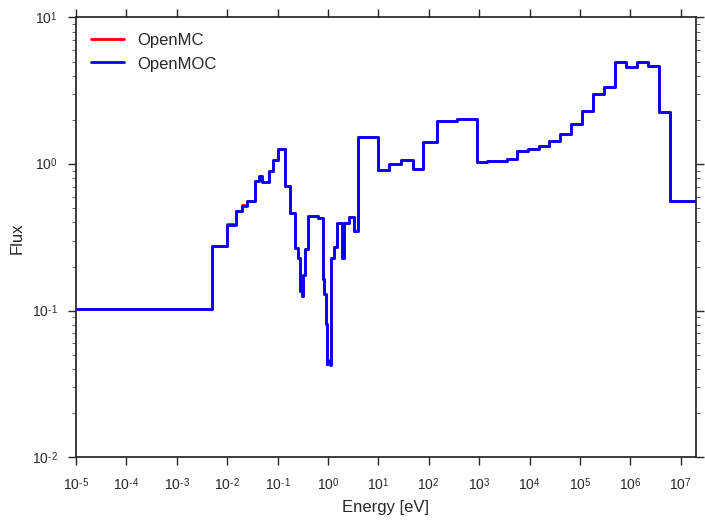
\includegraphics[width=\linewidth]{figures/biases/slab/vol-avg-flux}
  \caption{}
\end{subfigure}
\begin{subfigure}{0.9\textwidth}
  \centering
  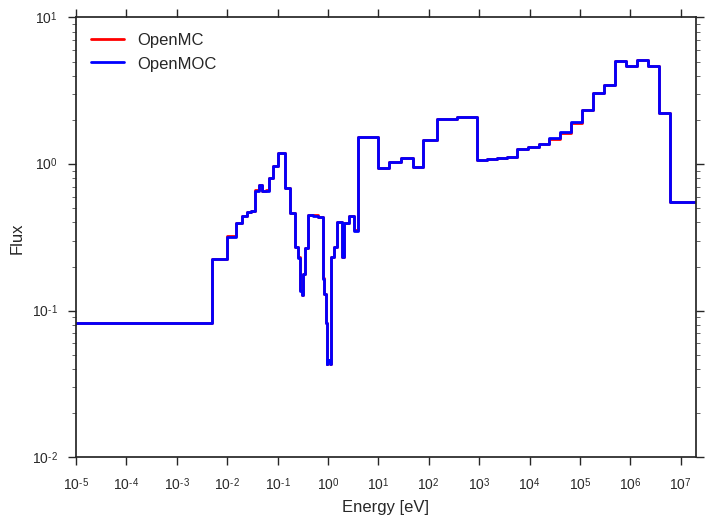
\includegraphics[width=\linewidth]{figures/biases/pin-cell/vol-avg-flux}
  \caption{}
\end{subfigure}
\caption[Flux spectrum in a slab and pin cell]{The flux spectrum in energy in a 1D slab (a) and 2D fuel pin (b).}
\label{fig:chap5-flux}
\end{figure}

%%%%%%%%%%%%%%%%%%%%%%%%%%%%%%%%%%%%%%%%
\subsection{Energy-Dependent Flux Error}
\label{subsec:chap5-diagnosis-energy}

Upon further inspection, it was noted that OpenMOC's flux exhibited large errors with respect to the reference OpenMC flux in those energy groups which isolate large U-238 capture resonances. The error in the 70-group flux is illustrated in Fig.~\ref{fig:chap5-rel-err-energy} for the \ac{FSR}s nearest and furthest from the moderator. These plots were generated for the benchmark models with a 16$\times$ \ac{FSR} discretization with \ac{MGXS} tallied on the \ac{FSR} mesh. The plots correspond to the case studies in Tables~\ref{table:chap5-slab-space} and~\ref{table:chap5-pin-space} with iso-in-lab scattering.

\begin{figure}[h!]
\begin{subfigure}{.9\textwidth}
  \centering
  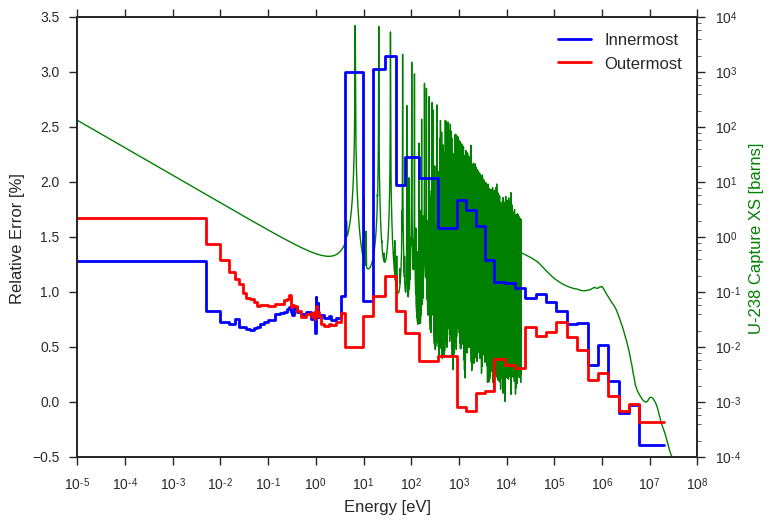
\includegraphics[width=\linewidth]{figures/biases/slab/rel-err-inner-outer}
  \caption{}
\end{subfigure}
\begin{subfigure}{.9\textwidth}
  \centering
  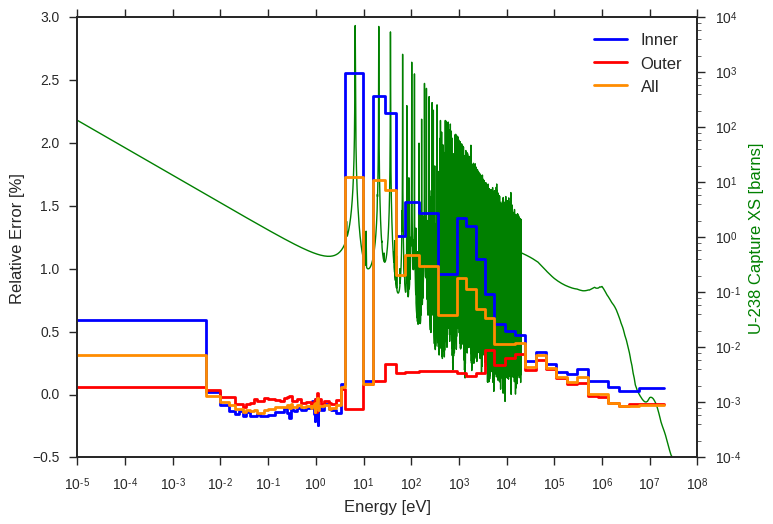
\includegraphics[width=\linewidth]{figures/biases/pin-cell/rel-err-inner-outer}
  \caption{}
\end{subfigure}
\caption[Flux relative error by energy group]{The energy-dependent relative error of the OpenMOC scalar flux with respect to the reference OpenMC flux in a 1D slab (a) and 2D fuel pin (b). The results correspond to the case studies presented in Tables~\ref{table:chap5-slab-space} and~\ref{table:chap5-pin-space}.}
\label{fig:chap5-rel-err-energy}
\end{figure}

As illustrated in the figures, there is a striking error of up to 1.5\% for the fluxes in the slab and up to 2.5\% for the fuel pin in the innermost \ac{FSR} in groups 24, 25 and 27. In addition, the flux errors appear to ``build up'' as the energy decreases through the resonance range, and the magnitude of the capture resonances increase. The one notable exception to this is group 26 (4 -- 9.877 eV) which does not include a U-238 capture resonance. These observations stand in contrast to the flux errors in the outermost \ac{FSR} for which no remarkable trend can be discerned. The positive error in the flux in groups with large capture resonances indicates that capture reaction rates are over-predicted in those groups by OpenMOC, contributing to the negative bias in the eigenvalue. Furthermore, these results indicate a strong relationship between the energy and spatial distribution of the flux errors, as is explored in the following section.

%\begin{emphbox}
%\textbf{The OpenMOC flux exhibits a few percent error in groups with large U-238 capture resonances.}
%\end{emphbox}

%%%%%%%%%%%%%%%%%%%%%%%%%%%%%%%%%%%%%%%%%%%
\subsection{Spatially-Dependent Flux Error}
\label{subsec:chap5-diagnosis-space}

The results presented in Fig.~\ref{fig:chap5-rel-err-energy} indicate significant errors in resonance groups, and in particular, group 27 in the 70-group calculation. Furthermore, the results indicated a large difference in the error profile for those \ac{FSR}s nearest and furthest from the moderator. These trends were studied further to better understand the spatial variation of the flux error across the 16 \ac{FSR}s in the fuel for the slab and pin geometries. In this analysis, the error of the flux was considered in the three different \textit{ranges} of energy group structures itemized below:

\vspace{-0.15cm}
\begin{itemize}[noitemsep]
  \item {\bf Range A} -- group 27 encompassing the U-238 capture resonance at 6.67 eV
  \item {\bf Range B} -- groups 11 -- 27 spanning the resonance range from 4 eV -- 408.5 keV
  \item {\bf Range C} -- groups 1 -- 70 spanning the entire energy regime from 0 -- 20 MeV
\end{itemize}
\vspace{-0.15cm}

Fig.~\ref{fig:chap5-rel-err-space} highlights the spatial dependence of the error across the fuel for each energy range. These plots were generated for the benchmark models with a 16$\times$ \ac{FSR} discretization with \ac{MGXS} tallied on the \ac{FSR} mesh. The plots correspond to the case studies in Tables~\ref{table:chap5-slab-space} and~\ref{table:chap5-pin-space} with iso-in-lab scattering.

The range A error in the slab monotonically decreases from a maximum of nearly 1.5\% to a minimum of $\sim$-0.5\% in those \ac{FSR}s furthest and nearest the moderator, with a similar trend observed for the fuel pin. Furthermore,  the trend accelerates in outermost 3--4 \ac{FSR}s nearest the moderator, where the error drops by nearly half of its value at the center of the slab and pin. The error profiles for energy ranges B and C exhibit the same decreasing trend from the inside to the oustide of the slab and pin, but the error magnitude never exceeds 0.5\% in magnitude. The systematic error trends in energy and space imply that the negative eigenvalue bias is driven by a poor prediction of the reaction rates in resonance groups, as investigated in the following section.

\begin{figure}[H]
\begin{subfigure}{.9\textwidth}
  \centering
  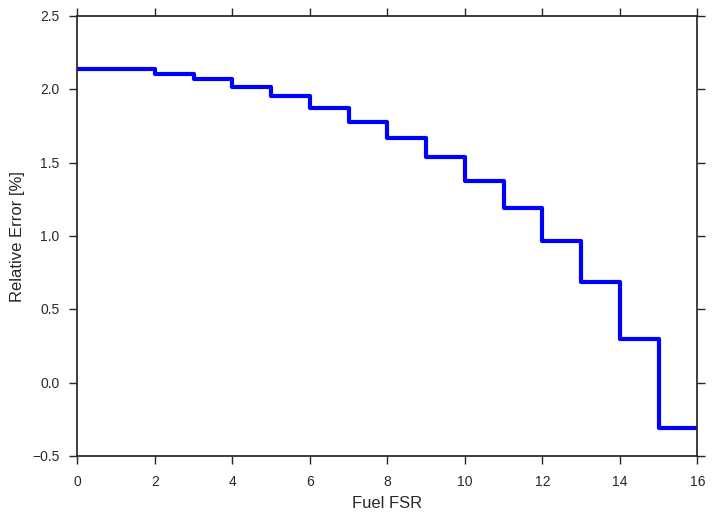
\includegraphics[width=\linewidth]{figures/biases/slab/rel-err-fuel-fsrs}
  \caption{}
\end{subfigure}
\begin{subfigure}{.9\textwidth}
  \centering
  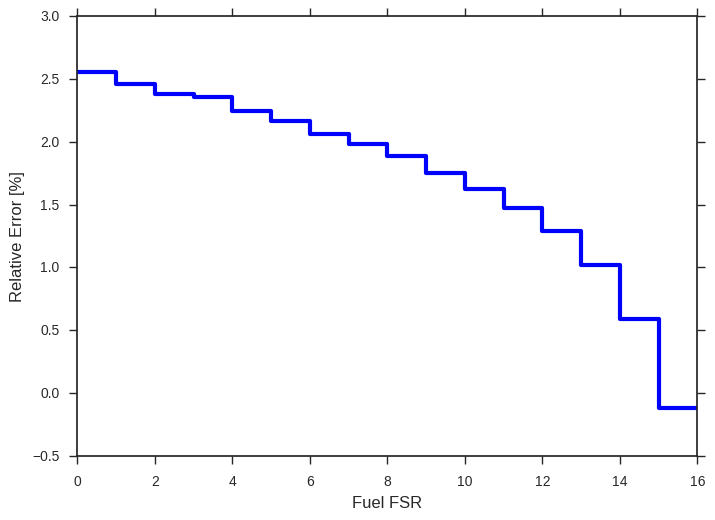
\includegraphics[width=\linewidth]{figures/biases/pin-cell/rel-err-fuel-fsrs}
  \caption{}
\end{subfigure}
\caption[Flux relative error by FSR]{The spatially-varying relative error of the OpenMOC scalar flux with respect to the reference OpenMC flux for a 1D slab (a) and 2D fuel pin (b) in group 27. The results correspond to Tables~\ref{table:chap5-slab-space} and~\ref{table:chap5-pin-space}.}
\label{fig:chap5-rel-err-space}
\end{figure}

%\begin{emphbox}
%\textbf{The flux error varies across the fuel in the slab and pin, and is greatest in those \ac{FSR}s nearest the center of the slab and fuel pin.}
%\end{emphbox}

%%%%%%%%%%%%%%%%%%%%%%%%%%%%%%%%%
\subsection{Reaction Rate Errors in the Resonance Regime}
\label{subsec:chap5-diagnosis-rxn-rates}

The errors in the multi-group flux directly correspond to equal errors in the reaction rates since the \ac{MGXS} are computed from the reference reaction rate and flux tallies. The results presented in Figs.~\ref{fig:chap5-rel-err-energy} and \ref{fig:chap5-rel-err-space} revealed significant errors in resonance groups, and in particular, group 27 in the 70-group calculation. In this section, the capture and absorption rate errors are evaluated to quantify how much of the negative eigenvalue bias in the two geometries can be attributed to the mis-predicted reaction rates in the resonance groups. This analysis was performed for different energy group structures to determine if errors in the reaction rates emerge with more energy groups, similar to the eigenvalue bias observed in the case studies in Sec.~\ref{sec:chap5-case-studies}.

The relative error for both U-238 capture and total absorption for all nuclides is quantified in Tab.~\ref{table:chap5-rxn-rate-errors} for energy ranges A, B and C (see Sec.~\ref{subsec:chap5-diagnosis-space}). As in Secs.~\ref{subsec:chap5-diagnosis-energy} and~\ref{subsec:chap5-diagnosis-space}, the analysis considered the slab and fuel pin benchmark models with a 16$\times$ \ac{FSR} discretization with \ac{MGXS} tallied on the \ac{FSR} mesh. The OpenMC iso-in-lab scattering feature was used to generate \ac{MGXS} for OpenMOC.

As illustrated in the table, the U-238 capture and total absorption rate errors each grow with the number of energy groups. This trend is particularly pronounced for U-238 capture in the 6.67 eV resonance group which approaches 0.6\% and 1.35\% for the slab and pin, respectively, when 25 or more groups are used in the multi-group calculation. The 0.08\% and 0.17\% error in the total absorption in range C directly corresponds to an under-prediction in the eigenvalue of 115 and 197 \ac{pcm} for the slab and fuel pin, respectively, which closely matches the observed eigenvalue bias for each model\footnote{This analysis neglects the contribution of scattering multiplicity (\textit{e.g.,} (n,xn)) to the eigenvalue.}. Approximately 5 -- 6\% and 16 -- 18\% of the total absorption occurs in energy ranges A and B, with U-238 capture accounting for 80\% and 70\% of the total absorption in each energy range, respectively. Hence, the error in U-238 resonance capture alone under-predicts the eigenvalue by 105 and 145 \ac{pcm} for the slab and pin, with approximately half of the error deriving from group 27 of 70 due to the resonance at 6.67 eV. 

%U-238 capture
%slab 27: 50 pcm
%slab all: 105 pcm
%pin 27: 100 pcm
%pin all: 185 pcm

%The total energy-integrated fission rate error is $\sim$1\% and $\sim$0.25\% for the slab and pin (and over 2\% in group 27) which would correspond to an over-prediction in the eigenvalue of

%Taken together, the errors in the absorption and fission rates would result in an eigenvalue bias that compares closely with the observed $\Delta\rho \approx$ 300 -- 350 \ac{pcm} \footnote{This analysis neglects the contribution of scattering multiplicity (\textit{e.g.,} (n,2n)) to the eigenvalue.}.

%Fig.~\ref{fig:chap5-pin-fuel-fsrs} highlights the spatial dependence of the error in group 27 across the fuel which isolates the largest U-238 capture resonance at 6.67 eV. The error decreases from a maximum of $\sim$2.8\% to a minimum of $\sim$0.6\% in those \ac{FSR}s furthest and nearest the moderator, respectively. It is unclear why the spatial dependence of the error does not monotonically decrease across the fuel pin as it does for the slab (see Fig.~\ref{fig:chap5-slab-fuel-fsrs}), but the overall trend is the same.

{\setlength{\extrarowheight}{-5pt}
\begin{table}[H]
  \centering
  \caption[Reaction rate relative errors]{The volume-integrated U-238 capture and total absorption rate percent relative errors. The errors correspond to the results in Tables~\ref{table:chap5-slab-space} and \ref{table:chap5-pin-space}.}
  \small
  \label{table:chap5-rxn-rate-errors} 
  \vspace{6pt}
  \begin{tabular}{| q | S[table-format=5.1] S[table-format=5.1] S[table-format=5.1] | S[table-format=5.1] S[table-format=5.1] S[table-format=5.1] |}
  \hhline{~|------|}
  \multicolumn{1}{c|}{\cellcolor{white}} &
  \multicolumn{3}{c|}{\cellcolor{lightgray} {\bf U-238 Capture}} &
  \multicolumn{3}{c|}{\cellcolor{lightgray} {\bf Total Absorption}} \\
  \multicolumn{1}{c|}{\cellcolor{white}} &
  {\bf \cellcolor{lightgray} Range A} &
  {\bf \cellcolor{lightgray} Range B} &
  {\bf \cellcolor{lightgray} Range C} &
  {\bf \cellcolor{lightgray} Range A} &
  {\bf \cellcolor{lightgray} Range B} &
  {\bf \cellcolor{lightgray} Range C} \\
  \midrule
  \multicolumn{1}{|c|}{\cellcolor{lightgray} {\bf \# Groups}} &
  \multicolumn{6}{c|}{\cellcolor{carolinablue} {\bf 1D Slab}} \\
  \hhline{~|------|}
1 & -0.02 & -0.02 & -0.02 & -0.11 & -0.11 & -0.11 \\
2 & 0.05 & 0.05 & 0.03 & 0.05 & 0.05 & -0.07 \\
4 & 0.11 & -0.08 & 0.06 & 0.12 & -0.08 & -0.05 \\
8 & 0.19 & -0.03 & 0.11 & 0.22 & -0.03 & 0.00 \\
16 & 0.21 & -0.02 & 0.12 & 0.23 & -0.02 & 0.02 \\
25 & 0.58 & 0.36 & 0.26 & 0.61 & 0.37 & 0.06 \\
40 & 0.58 & 0.43 & 0.30 & 0.61 & 0.44 & 0.07 \\
70 & {\cellcolor{darktangerine}} 0.59 & 0.46 & 0.30 & 0.61 & 0.47 & 0.08 \\
  \midrule
  \multicolumn{1}{c|}{\cellcolor{white}} & 
  \multicolumn{6}{c|}{\cellcolor{lightgreen} {\bf 2D Fuel Pin}} \\
  \midrule
1 & -0.02 & -0.02 & -0.02 & -0.07 & -0.07 & -0.07 \\
2 & 0.11 & 0.11 & 0.07 & 0.11 & 0.11 & -0.03 \\
4 & 0.55 & 0.07 & 0.32 & 0.54 & 0.07 & 0.04 \\
8 & 0.71 & 0.11 & 0.40 & 0.72 & 0.11 & 0.08 \\
16 & 0.72 & 0.12 & 0.41 & 0.73 & 0.12 & 0.09 \\
25 & 1.32 & 0.85 & 0.61 & 1.34 & 0.85 & 0.15 \\
40 & 1.33 & 0.93 & 0.64 & 1.34 & 0.92 & 0.16 \\
70 & {\cellcolor{darktangerine}} 1.33 & 0.99 & 0.65 & 1.35 & 0.97 & 0.17 \\
  \bottomrule
\end{tabular}
\end{table}}

These results indicate that spatial self-shielding effects in resonance groups is not adequately captured by the \ac{MGXS} and/or the multi-group calculation. Furthermore, this analysis illustrates the counter-intuitive result that the bias between continuous energy Monte Carlo and multi-group deterministic transport may in fact increase in magnitude with more energy groups. Although it is challenging to isolate the factors which convolve to bias the eigenvalue, the data presented here indicates that an over-prediction of U-238 capture in the resonance groups largely drives the error. These results will be discussed in greater depth in the context of angular-dependent \ac{MGXS} in Chapter~\ref{chap:sph}.

\begin{emphbox}
\textbf{The negative eigenvalue bias is caused by an over-prediction of absorption, dominated by U-238 capture in the 6.67 eV resonance. The reaction rate error increases with more energy groups as observed for the eigenvalue bias.}
\end{emphbox}

\clearpage

\vfill
\begin{highlightsbox}[frametitle=Highlights]
\begin{itemize}
  \item OpenMOC calculations were performed using \ac{MGXS} generated by OpenMC to compare eigenvalues for simple benchmarks.
  \item The eigenvalues closely agreed for homogeneous infinite media. The eigenvalues exhibited a bias of -200 to -300 \ac{pcm} for heterogenous geometries, including a 1D slab and 2D fuel pin.
  \item A series of case studies demonstrated the dependence of the bias with:
  \begin{itemize}
%    \item \textit{\ac{FSR} discretization} -- The bias was jointly-dependent with energy group structure.
    \item \textit{Energy condensation} -- The bias increased with more energy groups due to systematic errors in groups with large U-238 capture resonances.
    \item \textit{Spatial homogenization} -- The spatial tally mesh used to generate \ac{MGXS} in the fuel and moderator had no effect on the bias.
    \item \textit{Angular treatment} -- \ac{MGXS} generated with iso-in-lab scattering in OpenMC reduced the bias by $<$100 \ac{pcm} or $\sim\frac{1}{3}$.
  \end{itemize} 
  \item The eigenvalue bias is largely attributable to an over-prediction of U-238 capture rates in resonance groups.
  \item The flux errors indicate that spatial self-shielding is not adequately modeled in spatially heterogeneous multi-group calculations even when the ``true'' scalar flux is used to compute \ac{MGXS}.
\end{itemize}
\end{highlightsbox}
\vfill